
\documentclass[11pt,a4paper]{article}
\usepackage[margin=0.88in]{geometry}
\usepackage{amsmath,amssymb,amsthm,mathtools}
\usepackage{booktabs,array,tabularx,longtable,multirow}
\usepackage{graphicx,float}
\usepackage{xcolor}
\usepackage{enumitem}
\usepackage{hyperref}
\usepackage{xurl}
\usepackage[numbers]{natbib}
\usepackage{tikz}
\usetikzlibrary{arrows.meta,positioning,fit,calc,shapes.geometric,backgrounds}
\usepackage{pgfplots}
\pgfplotsset{compat=1.18}
\usepackage{caption}
\usepackage{microtype}
\hypersetup{colorlinks=true,linkcolor=blue!55!black,citecolor=blue!55!black,urlcolor=blue!55!black}
\setlength{\parskip}{0.38em}
\setlength{\parindent}{0pt}
\renewcommand{\arraystretch}{1.12}
\newcommand{\R}{\mathbb{R}}
\newcommand{\E}{\mathbb{E}}
\newcommand{\one}{\mathbf{1}}
\newcommand{\argmax}{\operatorname*{arg\,max}}
\newcommand{\argmin}{\operatorname*{arg\,min}}
\definecolor{nyuviolet}{RGB}{87,6,140}
\definecolor{deepblue}{RGB}{35,65,120}
\definecolor{darkgreen}{RGB}{25,110,70}
\tikzset{layer/.style={rectangle, rounded corners=3pt, draw=nyuviolet!75, very thick, fill=nyuviolet!6, align=center, minimum height=0.78cm, text width=2.75cm}, optbox/.style={rectangle, rounded corners=2pt, draw=deepblue!70, thick, fill=deepblue!5, align=center, minimum height=0.65cm, text width=3.1cm}, arrow/.style={-{Latex[length=2.5mm]}, thick, draw=black!65}, heatcell/.style={rectangle, minimum width=3.15cm, minimum height=0.70cm, draw=white, line width=0.9pt, font=\small\bfseries, align=center}}

\title{\textbf{Portfolio Allocation as Layered System Optimization:}\\ Mathematical Modeling, Control Decomposition, and Empirical Evaluation}
\author{Ashesh Kaji\\\textit{System Optimization Methods, New York University}\\\href{mailto:ask9184@nyu.edu}{ask9184@nyu.edu}}
\date{April 2026}
\begin{document}
\maketitle

\begin{abstract}
This report presents the portfolio-allocation project explicitly as a System Optimization Methods study. Rather than treating the empirical work as a collection of finance backtests, the paper models allocation as a sequential stochastic control problem with discrete universe and screen decisions, continuous portfolio weights, transaction-cost control effort, and a learned meta-controller. The mathematical starting point is the Markowitz convex mean--variance program, extended through turnover-regularized optimal control, cardinality-constrained screening, online model selection, and policy-gradient reinforcement learning. The final empirical study evaluates this layered formulation on liquid U.S. equity candidate universes of increasing breadth. The central result is that the optimal control stack is not invariant: a top-100 candidate set favors a 21-day momentum screen followed by equal weighting, a top-250 set favors low-volatility screening followed by equal weighting, and a top-500 set favors volatility-adjusted momentum followed by short-horizon rank-and-hold weighting. A policy-gradient router over the same screen/controller arms recovers stable and interpretable policies, but does not dominate a simple trailing-window adaptive rule. The contribution is therefore methodological as much as empirical: the project shows how convex optimization, combinatorial screening, online control, and reinforcement learning can be integrated into a single layered allocation system, and it identifies where each optimization layer adds value or fails to justify its complexity.
\end{abstract}

\section{Motivation: Why This Is a System Optimization Problem}
The project began from the classical convex portfolio optimization problem: estimate expected returns $\mu\in\R^n$ and covariance $\Sigma\succeq0$, then solve
\begin{equation}
\begin{aligned}
\max_{w\in\R^n}\quad & \mu^\top w - \lambda w^\top \Sigma w\\
\text{s.t.}\quad & \one^\top w = 1,\qquad w\ge 0.
\end{aligned}
\label{eq:markowitz}
\end{equation}
This model is a natural starting point for a system optimization course because it is a convex quadratic program on the simplex. But it is not a sufficient model of a live allocation system. In practice, a portfolio controller must repeatedly solve a decision problem under uncertainty, update its active set, trade off exploitation against turnover, and decide whether the controller itself should change when the opportunity set changes.

The study therefore treats portfolio allocation as a closed-loop system. At each rebalance time $t$, the system observes market information $\mathcal{F}_t$, chooses a candidate universe $\mathcal{U}_t$, applies a screen $S_t$, chooses a weighting controller $C_t$, executes a portfolio $w_t$, and observes net reward after transaction costs. The resulting problem combines four optimization types:
\begin{enumerate}[leftmargin=1.5em]
    \item \textbf{Convex optimization:} continuous weight selection under risk and turnover penalties.
    \item \textbf{Combinatorial optimization:} cardinality-constrained subset selection over candidate securities.
    \item \textbf{Sequential control:} repeated portfolio adjustment under path-dependent transaction costs.
    \item \textbf{Online learning / reinforcement learning:} adaptive routing among screen/controller arms.
\end{enumerate}
The purpose of the final experiment is to determine which layer is doing useful work and when extra optimization complexity is justified.

\section{From Static Convex Optimization to Dynamic Control}
\subsection{Single-period convex model}
The Markowitz problem in Equation~\eqref{eq:markowitz} is convex after converting the maximization into minimization:
\begin{equation}
\min_{w\in\Delta_n}\; \lambda w^\top \Sigma w - \mu^\top w, \qquad \Delta_n=\{w:\one^\top w=1,\; w\ge0\}.
\end{equation}
It provides a clean language for risk aversion and diversification. The Lagrangian for the equality-constrained, unconstrained-sign version is
\begin{equation}
\mathcal{L}(w,\eta)=\lambda w^\top\Sigma w-\mu^\top w + \eta(\one^\top w-1),
\end{equation}
with first-order condition
\begin{equation}
2\lambda \Sigma w - \mu + \eta\one =0.
\end{equation}
This condition shows the central optimization tradeoff: weights tilt toward expected return only insofar as covariance-scaled risk permits. However, the empirical project repeatedly showed that estimating $\mu$ and $\Sigma$ is only one part of the decision. A controller can fail not because the convex program is badly solved, but because the universe or active set is not aligned with the signal being optimized.

\subsection{Turnover as control effort}
The first operational extension is to add trading friction. Let $w_{t^-}$ be the portfolio before rebalancing and $w_t$ the target portfolio. A proportional transaction-cost model is
\begin{equation}
\text{TC}_t = \kappa \lVert w_t-w_{t^-}\rVert_1,
\end{equation}
where $\kappa$ is the one-way cost rate. The corresponding turnover-regularized convex controller is
\begin{equation}
\begin{aligned}
\max_{w_t\in\Delta_n}\quad & \alpha_t^\top w_t - \lambda w_t^\top\widehat{\Sigma}_t w_t - \gamma\lVert w_t-w_{t^-}\rVert_1.
\end{aligned}
\label{eq:turnover_convex}
\end{equation}
Equation~\eqref{eq:turnover_convex} connects directly to dynamic trading models with transaction costs: the current position becomes part of the state, and turnover becomes control effort. Even when a rank-based controller rather than a full convex QP is used, the same control-cost logic remains central because high-churn rank-and-hold policies lose more to friction.

\subsection{Sequential objective}
The live problem is finite-horizon stochastic optimal control:
\begin{equation}
\max_{\pi}\; \E_\pi\left[\sum_{t=0}^{T-1}\delta^t\left(w_t^\top r_{t+1}-\kappa\lVert w_t-w_{t^-}\rVert_1-\rho\,\mathcal{R}(w_t,\mathcal{F}_t)\right)\right],
\label{eq:sequential_objective}
\end{equation}
where $w_t$ is the post-trade portfolio, $w_{t^-}$ is the pre-trade portfolio, $r_{t+1}$ is the next-period return vector, $\kappa$ is the transaction-cost coefficient, $\rho$ is a risk-penalty coefficient, $\pi$ maps observed state to actions, $\delta$ is a discount factor, and $\mathcal{R}$ is a risk or instability penalty. If the transition model were known, the corresponding Bellman recursion could be written by setting $x_t=(\mathcal{F}_t,w_{t^-})$, $a_t=w_t$, and
\begin{equation}
g(x_t,a_t)=\E\!\left[w_t^\top r_{t+1}\mid\mathcal{F}_t\right]-\kappa\lVert w_t-w_{t^-}\rVert_1-\rho\,\mathcal{R}(w_t,\mathcal{F}_t),
\end{equation}
so that
\begin{equation}
V_t(x_t)=\max_{a_t\in\mathcal{A}(x_t)}\left\{g(x_t,a_t)+\delta\E[V_{t+1}(x_{t+1})\mid x_t,a_t]\right\}.
\end{equation}
Here $\mathcal{A}(x_t)$ encodes the admissible portfolio simplex, eligibility, leverage, and turnover constraints, with terminal value normalized as $V_T(x_T)=0$ for the finite-horizon evaluation used in the backtests.
The implemented study approximates this ideal control problem through interpretable policy classes: screens, rank-and-hold rules, equal weighting, and learned routing. The empirical question is not whether the theoretical Bellman equation can be solved exactly; it is whether decomposition into tractable subproblems produces better and more interpretable allocation decisions.

\section{Layered Mathematical Formulation}
\subsection{Bilevel mixed discrete-continuous view}
Let $b\in\{100,250,500\}$ index candidate-universe breadth, $j\in\mathcal{J}$ index a screen, and $k\in\mathcal{K}$ index a weighting controller. The full model-selection problem can be written as
\begin{equation}
\begin{aligned}
\max_{b,j,k}\quad & \frac{\widehat{\mu}_{b,j,k}}{\widehat{\sigma}_{b,j,k}} - \phi\,\widehat{\text{DD}}_{b,j,k} - \psi\,\widehat{\text{TO}}_{b,j,k}\\
\text{s.t.}\quad & H_{b,j}(t)=S_j(\mathcal{U}_b(t),\mathcal{F}_t),\\
& w_t=C_k(H_{b,j}(t),\mathcal{F}_t,w_{t^-}),\\
& |H_{b,j}(t)|\le K_{\max},\qquad w_t\in\Delta_{|H_{b,j}(t)|}.
\end{aligned}
\label{eq:bilevel_stack}
\end{equation}
Here $\widehat{\mu}_{b,j,k}$, $\widehat{\sigma}_{b,j,k}$, $\widehat{\text{DD}}_{b,j,k}$, and $\widehat{\text{TO}}_{b,j,k}$ are walk-forward estimates of mean return, volatility, drawdown, and turnover for the stack $(b,j,k)$. This is not a single convex program. It is a mixed discrete-continuous model-selection problem with lower-level portfolio maps embedded in $C_k$. The empirical design makes it tractable by enumerating a disciplined grid of $(b,j,k)$ arms, evaluating each arm out of sample, and then studying the performance surface.

\begin{figure}[H]
\centering
\resizebox{0.98\textwidth}{!}{%
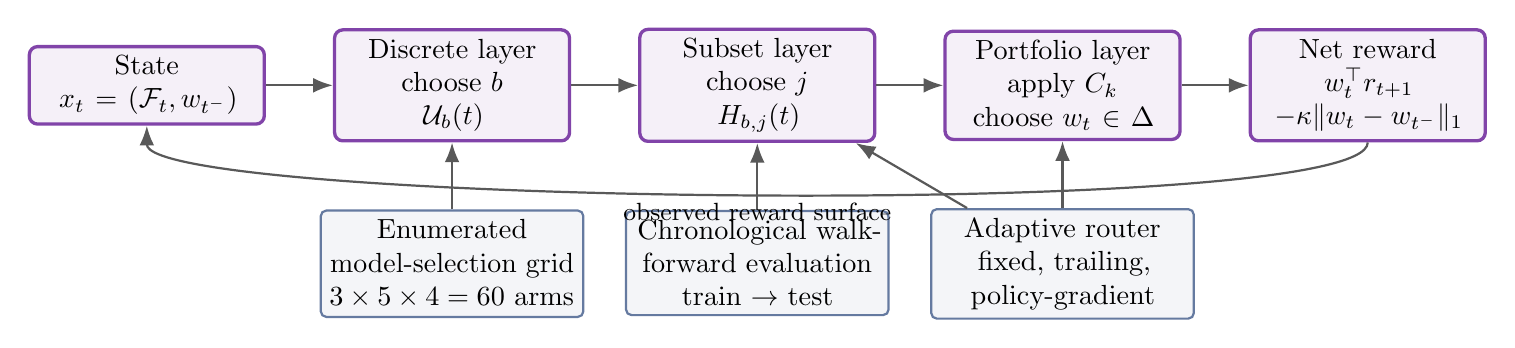
\begin{tikzpicture}[node distance=0.65cm and 0.85cm]
\node[layer] (state) {State\\$x_t=(\mathcal{F}_t,w_{t^-})$};
\node[layer, right=of state] (universe) {Discrete layer\\choose $b$\\$\mathcal{U}_b(t)$};
\node[layer, right=of universe] (screen) {Subset layer\\choose $j$\\$H_{b,j}(t)$};
\node[layer, right=of screen] (weights) {Portfolio layer\\apply $C_k$\\choose $w_t\in\Delta$};
\node[layer, right=of weights] (reward) {Net reward\\$w_t^\top r_{t+1}$\\$-\kappa\|w_t-w_{t^-}\|_1$};
\node[optbox, below=0.85cm of universe] (enumerate) {Enumerated model-selection grid\\$3\times5\times4=60$ arms};
\node[optbox, below=0.85cm of screen] (wf) {Chronological walk-forward evaluation\\train $\rightarrow$ test};
\node[optbox, below=0.85cm of weights] (router) {Adaptive router\\fixed, trailing, policy-gradient};
\draw[arrow] (state)--(universe);
\draw[arrow] (universe)--(screen);
\draw[arrow] (screen)--(weights);
\draw[arrow] (weights)--(reward);
\draw[arrow] (enumerate)--(universe);
\draw[arrow] (wf)--(screen);
\draw[arrow] (router)--(screen);
\draw[arrow] (router)--(weights);
\draw[arrow] (reward.south) .. controls +(0,-1.0) and +(0,-1.0) .. node[below,font=\small]{observed reward surface} (state.south);
\end{tikzpicture}}
\caption{Optimization decomposition used in the study. A difficult mixed discrete-continuous sequential problem is decomposed into enumerated universe/screen/controller arms, walk-forward evaluation, and an adaptive routing layer.}
\label{fig:decomposition}
\end{figure}

\subsection{Screens as constrained projections}
Each screen is a set-valued map from the candidate universe into a smaller active set:
\begin{equation}
S_j:\left(\mathcal{U}_b(t),\mathcal{F}_t\right)\mapsto H_{b,j}(t),\qquad |H_{b,j}(t)|\le K_{\max}.
\end{equation}
For a score $q_i(t)$, the top-$K$ screen solves the cardinality problem
\begin{equation}
\max_{z\in\{0,1\}^{|\mathcal{U}|}}\; \sum_{i\in\mathcal{U}} q_i(t)z_i
\quad\text{s.t.}\quad \sum_i z_i\le K.
\label{eq:topk}
\end{equation}
The five score functions tested are
\begin{align}
q_i^{\text{mom},\tau}(t) &= P_i(t)/P_i(t-\tau)-1,\\
q_i^{\text{vam},\tau}(t) &= \frac{P_i(t)/P_i(t-\tau)-1}{\widehat{\sigma}_{i,\tau}(t)+\epsilon},\\
q_i^{\text{lowvol},\tau}(t) &= -\widehat{\sigma}_{i,\tau}(t),\\
q_i^{\text{cluster}}(t) &= q_i^{\text{mom},63}(t)\quad\text{with per-cluster selection caps}.
\end{align}
This is where a major system-optimization insight enters the project: screening is not data cleaning. It is a discrete optimization layer that changes the feasible set available to every downstream controller.

\subsection{Weighting controllers as restricted policy classes}
After screening, the controller chooses weights on the active set $H_t$. Equal weighting is the minimum-estimation controller:
\begin{equation}
w_{i,t}=\frac{1}{|H_t|}\mathbf{1}\{i\in H_t\}.
\end{equation}
Rank-and-hold is another cardinality-constrained policy, now inside the screened set:
\begin{equation}
w_{i,t}=\frac{1}{k}\mathbf{1}\left\{i\in\operatorname{TopK}_{\ell\in H_t}\left(P_\ell(t)/P_\ell(t-\tau)-1\right)\right\}.
\label{eq:rank_hold}
\end{equation}
Although Equation~\eqref{eq:rank_hold} is simpler than a full quadratic program, it is still an optimization rule: it solves a top-$k$ linear ranking objective over the screened active set. The final study compares whether this extra active layer is worth its turnover cost after screening has already concentrated the universe.

\section{Learning and Meta-Control Formulation}
\subsection{Model selection as an online expert problem}
Let each screen/controller pair be an arm $a\in\mathcal{A}$ with realized reward $R_t(a)$ in walk-forward period $t$. A non-learning model-selection baseline chooses
\begin{equation}
a^{\text{train}}=\argmax_{a\in\mathcal{A}}\sum_{t\in\mathcal{T}_{\text{train}}}R_t(a)
\end{equation}
and holds that arm in the test period. The trailing-window router chooses
\begin{equation}
a_t^{\text{trail}}=\argmax_{a\in\mathcal{A}}\sum_{s=t-L}^{t-1}R_s(a),
\end{equation}
which is an online adaptive rule. This comparator is important because any learned method must beat simple, transparent online optimization before it can be considered practically useful.

\subsection{Policy-gradient router}
The reinforcement-learning router treats the arm-selection problem as a finite-action Markov decision process. The state $s_t$ contains time features, scope identity, trailing rewards, and the most recent reward vector. The policy is a softmax over arm logits:
\begin{equation}
\pi_\theta(a\mid s_t)=\frac{\exp(f_\theta(s_t)_a)}{\sum_{a'\in\mathcal{A}}\exp(f_\theta(s_t)_{a'})}.
\end{equation}
The reward is next-period net reward minus a switching penalty:
\begin{equation}
r_t^{\text{router}}=R_t(a_t)-\xi\mathbf{1}\{a_t\ne a_{t-1}\}.
\end{equation}
The policy-gradient update estimates
\begin{equation}
\nabla_\theta J(\theta)=\E_\pi\left[\sum_t (G_t-b_t)\nabla_\theta\log\pi_\theta(a_t\mid s_t)\right],
\label{eq:policy_gradient}
\end{equation}
where $G_t$ is a return-to-go and $b_t$ is a variance-reduction baseline. The important methodological choice is that reinforcement learning is not asked to learn raw portfolio weights from scratch. It is placed at the system level, where the action space consists of interpretable optimization stacks.

\section{Experimental Protocol as Optimization Evidence}
The final empirical matrix uses three universe scopes, five screens, and four weighting controllers, producing $3\times5\times4=60$ primary arms at the 10 basis point cost slice. Each arm is evaluated through chronology-respecting walk-forward splits: screen membership is computed using only information available through the training end date, and performance is measured on the subsequent evaluation interval. This is the empirical analogue of out-of-sample control evaluation.

\begin{table}[H]
\centering
\caption{Layer map of the optimization decomposition and its empirical instantiations.}
\label{tab:layer_map}
\small
\begin{tabularx}{\textwidth}{p{2.6cm}p{3.8cm}X}
\toprule
Layer & Mathematical role & Implementation in final study\\
\midrule
Universe breadth & Discrete state/action defining candidate feasible set & Top-100, top-250, and top-500 liquid-equity candidate scopes\\
Screen & Cardinality-constrained subset optimization & Momentum, volatility-adjusted momentum, low-volatility, cluster-capped momentum top-10 screens\\
Weighting & Continuous or restricted portfolio policy on simplex & Equal weight and 21/63/126-day rank-and-hold top-5 controllers\\
Trading friction & Control effort / path dependence & Net reward subtracts proportional turnover cost at 10 bps primary slice\\
Routing & Online model selection / MDP policy & Train-selected fixed arm, trailing-window router, random router, policy-gradient router, oracle bounds\\
Validation & Out-of-sample control evaluation & Chronological walk-forward splits, all-trials ledger, model-selection ledger, multiple-comparison diagnostic\\
\bottomrule
\end{tabularx}
\end{table}

\section{Optimization Results}
\subsection{Main solution stacks}
The strongest empirical evidence that the layered model matters is that the selected solution stack changes with universe breadth.
\begin{table}[H]
\centering
\caption{Best screen/controller stack by candidate-universe breadth. Values are mean walk-forward metrics at 10 bps transaction cost.}
\label{tab:winners_math}
\small
\resizebox{\textwidth}{!}{%
\begin{tabular}{lllrrrrr}
\toprule
Universe & Discrete screen solution & Weighting solution & Splits & Ann. ret. & Ann. vol. & Sharpe & Worst DD\\
\midrule
Top-100 & 21-day momentum top 10 & Equal weight & 22 & 20.4\% & 20.2\% & 1.474 & -44.9\%\\
Top-250 & 63-day low-volatility top 10 & Equal weight & 11 & 11.2\% & 14.1\% & 0.859 & -10.5\%\\
Top-500 & Vol.-adjusted 63-day momentum top 10 & 21-day rank-and-hold & 9 & 35.1\% & 20.8\% & 1.756 & -15.5\%\\
\bottomrule
\end{tabular}%
}
\end{table}
The optimization interpretation is direct. If the universe is narrow, screening already performs most of the selection and equal weighting is an adequate solution on the resulting simplex. In the broadest universe, the feasible set contains enough cross-sectional dispersion that a second ranking optimization inside the screened set improves risk-adjusted performance. In the intermediate universe, low-volatility screening dominates, suggesting that the best solution is to reduce noise rather than chase momentum.

\subsection{Screen layer: objective functions matter}
\begin{figure}[H]
\centering
\resizebox{0.98\textwidth}{!}{%
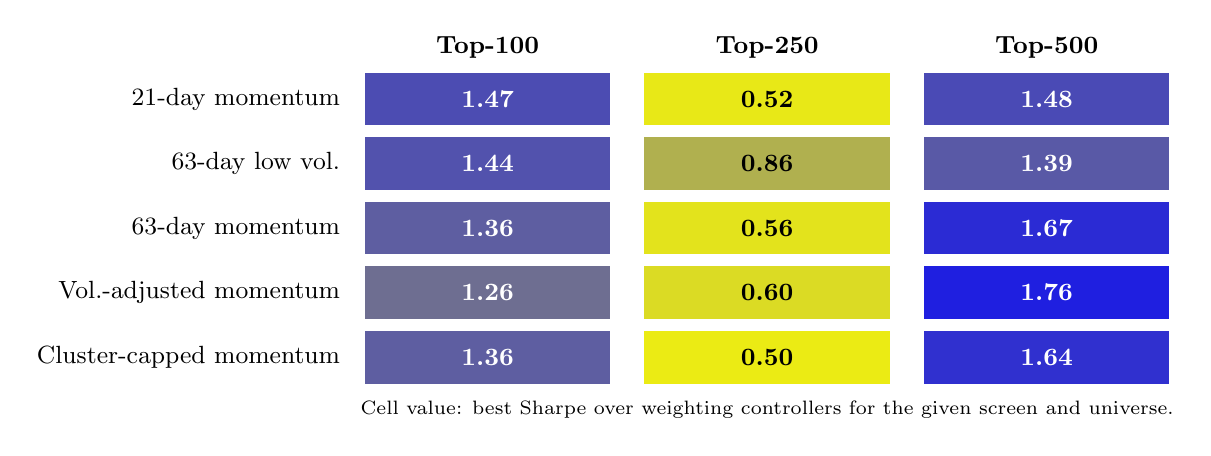
\begin{tikzpicture}
\node[heatcell, fill=blue!70!yellow, text=white] at (0.0,0.0) {1.47};
\node[heatcell, fill=blue!9!yellow, text=black] at (3.55,0.0) {0.52};
\node[heatcell, fill=blue!71!yellow, text=white] at (7.10,0.0) {1.48};
\node[heatcell, fill=blue!68!yellow, text=white] at (0.0,-0.82) {1.44};
\node[heatcell, fill=blue!31!yellow, text=black] at (3.55,-0.82) {0.86};
\node[heatcell, fill=blue!65!yellow, text=white] at (7.10,-0.82) {1.39};
\node[heatcell, fill=blue!63!yellow, text=white] at (0.0,-1.64) {1.36};
\node[heatcell, fill=blue!11!yellow, text=black] at (3.55,-1.64) {0.56};
\node[heatcell, fill=blue!83!yellow, text=white] at (7.10,-1.64) {1.67};
\node[heatcell, fill=blue!57!yellow, text=white] at (0.0,-2.46) {1.26};
\node[heatcell, fill=blue!14!yellow, text=black] at (3.55,-2.46) {0.60};
\node[heatcell, fill=blue!88!yellow, text=white] at (7.10,-2.46) {1.76};
\node[heatcell, fill=blue!63!yellow, text=white] at (0.0,-3.28) {1.36};
\node[heatcell, fill=blue!8!yellow, text=black] at (3.55,-3.28) {0.50};
\node[heatcell, fill=blue!81!yellow, text=white] at (7.10,-3.28) {1.64};
\foreach \j/\name in {0/{Top-100},1/{Top-250},2/{Top-500}} {\node[font=\small\bfseries, align=center] at (\j*3.55,0.65) {\name};}
\foreach \i/\name in {0/{21-day momentum},1/{63-day low vol.},2/{63-day momentum},3/{Vol.-adjusted momentum},4/{Cluster-capped momentum}} {\node[font=\small, anchor=east, align=right] at (-1.75,-\i*0.82) {\name};}
\node[font=\scriptsize, align=center] at (3.55,-3.95) {Cell value: best Sharpe over weighting controllers for the given screen and universe.};
\end{tikzpicture}}
\caption{Screen objective functions define different feasible active sets. The heatmap shows that the best screening objective changes by universe breadth.}
\label{fig:screen_heatmap_math}
\end{figure}
Figure~\ref{fig:screen_heatmap_math} is the most compact visual evidence that the screen is an optimization layer. The top-250 universe is weak across most momentum screens, but improves under the low-volatility objective. The top-500 universe rewards volatility-adjusted and medium-horizon momentum objectives. Thus, the screen objective changes the feasible set in a way that can dominate the weighting rule.

\subsection{Weighting layer: when extra control effort pays}
Averaging over screens, equal weighting has the best mean Sharpe in the top-100 and top-250 scopes, while 21-day rank-and-hold has the best mean Sharpe in the top-500 scope. This is a system-level cost-benefit result. Extra optimization effort is not universally valuable; it is valuable when the upstream feasible set is broad enough to contain exploitable dispersion.
\begin{table}[H]
\centering
\caption{Controller ablation: best weighting rule averaged over screens.}
\label{tab:controller_ablation_math}
\small
\resizebox{\textwidth}{!}{%
\begin{tabular}{llrrp{5.0cm}}
\toprule
Universe & Best controller by average screen Sharpe & Mean Sharpe & Best Sharpe & Interpretation\\
\midrule
Top-100 & Equal weight & 1.380 & 1.474 & screen does most selection\\
Top-250 & Equal weight & 0.572 & 0.859 & risk filtering beats active ranking\\
Top-500 & 21-day rank-and-hold & 1.433 & 1.756 & breadth justifies second control layer\\
\bottomrule
\end{tabular}
}
\end{table}
The turnover diagnostics support the same conclusion. Equal weight has essentially zero rebalance turnover after screen membership is fixed, while rank-and-hold rules introduce substantial turnover. When active ranking does not add enough signal, the turnover penalty makes the simpler controller superior.

\subsection{Model-selection risk and multiple comparisons}
Because each universe evaluates 20 screen/controller arms, a winning Sharpe must be interpreted as a selected maximum over many trials:
\begin{equation}
\widehat{a} = \argmax_{a\in\mathcal{A}} \widehat{\text{SR}}(a).
\end{equation}
The study therefore reports the winner gap against the second-best arm rather than presenting winners as formal statistical discoveries.
\begin{table}[H]
\centering
\caption{Exploratory multiple-comparison diagnostic. Gaps are descriptive, not p-values, because walk-forward folds overlap and arms are not independent.}
\label{tab:selection_risk_math}
\small
\begin{tabular}{lrrrr}
\toprule
Universe & Arms tested & Best Sharpe & Second Sharpe & Winner gap\\
\midrule
Top-100 & 20 & 1.474 & 1.440 & 0.034\\
Top-250 & 20 & 0.859 & 0.755 & 0.104\\
Top-500 & 20 & 1.756 & 1.666 & 0.090\\
\bottomrule
\end{tabular}
\end{table}
The top-100 winner is fragile because the gap is small. The top-250 and top-500 winners are more informative mechanically, but still should be treated as exploratory. This is why the paper emphasizes mechanisms--screen and controller ablations--rather than only selected winners.

\section{Reinforcement Learning as System-Level Optimization}
The learned router is evaluated as a meta-controller over already-interpretable optimization arms. This makes the RL component appropriate to the project: it is not a black-box replacement for portfolio theory, but a learned model-selection policy in a structured control system.

\begin{table}[H]
\centering
\caption{Integrated policy-gradient router results. Rewards are cumulative test-period rewards at the 10 bps cost slice; RL values are mean $\pm$ standard deviation over seven seeds for the best configuration.}
\label{tab:rl_math}
\scriptsize
\begin{tabular}{lrrrrrrrr}
\toprule
Scope & Test periods & RL & Train-fixed & Trailing & Random & Oracle & RL--fixed & RL--trailing\\
\midrule
Combined & 14 & 1.213 $\pm$ 0.063 & 1.134 & 1.543 & 1.276 & 2.586 & 0.079 & -0.330\\
Top-100 & 8 & 0.823 $\pm$ 0.011 & 0.827 & 0.475 & 0.657 & 1.355 & -0.004 & 0.348\\
Top-250 & 5 & 0.280 $\pm$ 0.068 & 0.305 & 0.306 & 0.296 & 0.764 & -0.026 & -0.026\\
Top-500 & 4 & 0.371 $\pm$ 0.000 & 0.371 & 0.566 & 0.525 & 0.932 & 0.000 & -0.196\\
\bottomrule
\end{tabular}
\end{table}
The RL results are academically useful precisely because they are not overclaimed. The policy-gradient router improves over the train-selected fixed arm in the combined panel and learns stable selections, but it does not dominate the trailing-window router. In optimization terms, the learned policy class and state representation are sufficient to recover some structure in the reward surface, but not sufficient to beat a low-complexity online optimizer that directly exploits recent realized rewards.

\begin{figure}[H]
\centering
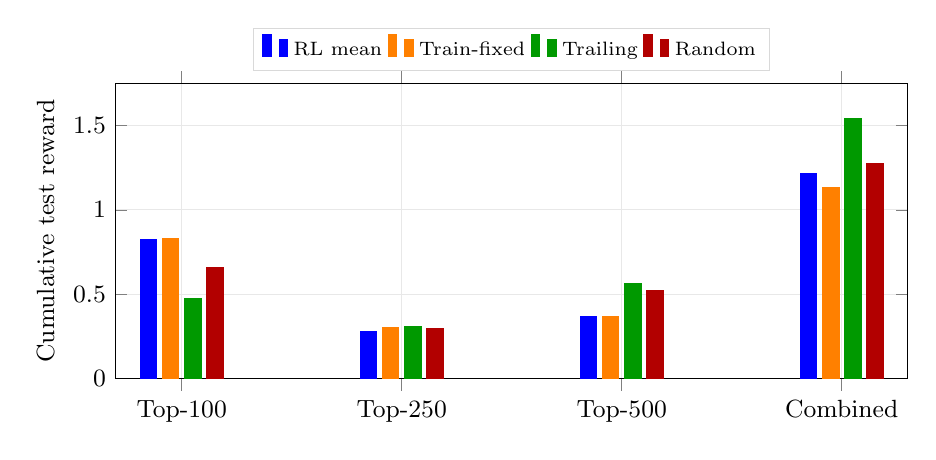
\begin{tikzpicture}
\begin{axis}[ybar,bar width=6pt,width=0.96\textwidth,height=0.44\textwidth,ylabel={Cumulative test reward},symbolic x coords={Top-100,Top-250,Top-500,Combined},xtick=data,ymin=0,ymax=1.75,grid=major,grid style={gray!18},legend style={at={(0.5,1.04)}, anchor=south, legend columns=4, font=\scriptsize, draw=gray!30},tick label style={font=\small},label style={font=\small}]
\addplot+[ybar, fill=blue, draw=blue] coordinates {(Top-100,0.823) (Top-250,0.280) (Top-500,0.371) (Combined,1.213)};
\addlegendentry{RL mean}
\addplot+[ybar, fill=orange, draw=orange] coordinates {(Top-100,0.827) (Top-250,0.305) (Top-500,0.371) (Combined,1.134)};
\addlegendentry{Train-fixed}
\addplot+[ybar, fill=green!60!black, draw=green!60!black] coordinates {(Top-100,0.475) (Top-250,0.306) (Top-500,0.566) (Combined,1.543)};
\addlegendentry{Trailing}
\addplot+[ybar, fill=red!70!black, draw=red!70!black] coordinates {(Top-100,0.657) (Top-250,0.296) (Top-500,0.525) (Combined,1.276)};
\addlegendentry{Random}
\end{axis}
\end{tikzpicture}
\caption{Adaptive model-selection comparison. The trailing-window rule is a strong online optimization baseline; the learned router is informative but not yet dominant.}
\label{fig:rl_math_bar}
\end{figure}

\section{How the Optimization Methods Shaped the Final Study}
The final experiment is not a finance study retrofitted into a systems class. It is the result of repeatedly translating portfolio ideas into optimization objects:
\begin{enumerate}[leftmargin=1.5em]
    \item The project began with Equation~\eqref{eq:markowitz}, a convex quadratic program, but empirical instability motivated simpler restricted policies and turnover-regularized objectives.
    \item Transaction costs converted static allocation into a path-dependent control problem, forcing the study to compare net rather than gross performance.
    \item Cardinality and universe construction converted the problem into a mixed discrete-continuous system, where feasible-set design can matter more than continuous weight optimization.
    \item Walk-forward evaluation turned backtesting into out-of-sample control validation rather than full-sample curve fitting.
    \item Reinforcement learning was integrated at the meta-control level, where the action space is structured and interpretable, rather than as an unconstrained black-box allocator.
\end{enumerate}
This progression is the central academic contribution. The mathematics was not ornamental; it determined what had to be measured. In particular, the layered formulation predicted that changing the feasible set could change the optimal controller, and the empirical study found exactly that.

\section{Limitations and Next Mathematical Step}
The main limitations are also optimization limitations. First, the candidate universes are not fully point-in-time, so the feasible sets $\mathcal{U}_b(t)$ are only approximations to investable historical universes. Second, the screen/controller grid is finite; it approximates the bilevel problem but does not solve the full mixed-integer program in Equation~\eqref{eq:bilevel_stack}. Third, the RL router has few independent test periods per scope, so policy-gradient results should be treated as exploratory. Fourth, market impact is modeled as proportional turnover rather than a nonlinear function of order size and liquidity.

The next rigorous step is not another broad sweep. It is to build point-in-time universe membership and rerun the layered system with more independent walk-forward episodes. Mathematically, this would improve the fidelity of the feasible set $\mathcal{U}_b(t)$ and provide enough samples to evaluate whether learned routing approximates the online model-selection optimum better than simple trailing-window selection.

\section{Conclusion}
This report reframes the final portfolio project as a layered system optimization study. The empirical conclusion is that the best allocation method is not just a weighting formula. It is a stack: universe construction, screen objective, weighting controller, and optional router. In the top-100 universe, the solution is simple: momentum screening plus equal weighting. In the top-250 universe, risk filtering is the useful optimization. In the top-500 universe, breadth creates enough dispersion for volatility-adjusted momentum plus short-horizon rank-and-hold to perform best. The learned router confirms that the hierarchy is learnable, but also demonstrates that a transparent trailing-window optimizer remains a difficult baseline.

For System Optimization Methods, the core lesson is that model formulation determines insight. Once portfolio allocation is modeled as a mixed discrete-continuous sequential control problem, the project stops being a search for a single best trading rule and becomes a study of where optimization should be applied: to the feasible set, to the weights, to the control cost, or to the routing policy. That is the practical and academic value of the final study.

\appendix
\section{Reproducibility Artifacts}
The primary run folder is \path{findings/2026-04-23-context-aware-grand-study/}. Key artifacts include:
\begin{itemize}[leftmargin=1.5em,noitemsep]
    \item \path{metrics/screened_core_summary.csv}, \path{metrics/screened_universe_winners.csv}, and \path{metrics/screen_ablation_summary.csv};
    \item \path{metrics/controller_ablation_summary.csv}, \path{metrics/multiple_testing_summary.csv}, and \path{metrics/integrated_rl_study_*.csv};
    \item \path{report/SYSTEM_OPTIMIZATION_METHODS_STUDY.tex} and \path{report/SYSTEM_OPTIMIZATION_METHODS_STUDY.pdf}.
\end{itemize}

\section{Controller and Screen Grid}
The core grid uses five screens: 21-day momentum top 10, 63-day momentum top 10, 63-day volatility-adjusted momentum top 10, 63-day low-volatility top 10, and 63-day cluster-capped momentum top 10. It uses four weighting controllers: equal weight, 21-day rank-and-hold top 5, 63-day rank-and-hold top 5, and 126-day rank-and-hold top 5. The primary reported cost slice is 10 basis points; 0 and 25 basis point slices are retained for cost-sensitivity diagnostics.

\bibliographystyle{plainnat}
\sloppy
\begin{thebibliography}{10}
\bibitem[Bailey and L{\'o}pez de Prado(2014)]{bailey2014deflated} Bailey, D.~H., and L{\'o}pez de Prado, M. (2014). The Deflated Sharpe Ratio: Correcting for Selection Bias, Backtest Overfitting, and Non-Normality. \textit{Journal of Portfolio Management}, 40(5), 94--107.
\bibitem[Cover(1991)]{cover1991universal} Cover, T.~M. (1991). Universal Portfolios. \textit{Mathematical Finance}, 1(1), 1--29.
\bibitem[DeMiguel et~al.(2009)]{demiguel2009optimal} DeMiguel, V., Garlappi, L., and Uppal, R. (2009). Optimal Versus Naive Diversification: How Inefficient is the 1/N Portfolio Strategy? \textit{Review of Financial Studies}, 22(5), 1915--1953.
\bibitem[G{\^a}rleanu and Pedersen(2013)]{garleanu2013dynamic} G{\^a}rleanu, N., and Pedersen, L.~H. (2013). Dynamic Trading with Predictable Returns and Transaction Costs. \textit{Journal of Finance}, 68(6), 2309--2340.
\bibitem[Markowitz(1952)]{markowitz1952portfolio} Markowitz, H. (1952). Portfolio Selection. \textit{Journal of Finance}, 7(1), 77--91.
\bibitem[Williams(1992)]{williams1992simple} Williams, R.~J. (1992). Simple Statistical Gradient-Following Algorithms for Connectionist Reinforcement Learning. \textit{Machine Learning}, 8(3), 229--256.
\bibitem[Zhang et~al.(2020)]{zhang2020deep} Zhang, Z., Zohren, S., and Roberts, S. (2020). Deep Reinforcement Learning for Trading. \textit{Journal of Financial Data Science}, 2(2), 25--40.
\end{thebibliography}
\end{document}
